\documentclass[12pt]{article}
\usepackage[utf8]{inputenc}
\usepackage[cm]{fullpage}
\usepackage{amssymb}
\usepackage{multicol}
\usepackage{graphicx}

%\usepackage{pgffor}   % for 'for loop' usage

%\usepackage{pstricks}

\newcommand{\exerc}[3]{ \vspace*{25pt} {$\mathbf{#1)}$} #2 \hfill {\it #3} }
\newcommand{\exitem}[2]{ \texttt{\bf #1)} #2 \\ }
\newcommand*\xor{\mathbin{\oplus}}

%\newcommand{\clock}[1]{
%    \psset{yunit=0.8}
%	\rput(0,0.1){
%      \foreach \n in {0,...,#1}{
%	  \translate(2,0)
%      \psline
%	    (0,0)(1,0)(1,1)(2,1)
%	  }
%	}
%    \psset{yunit=1.0}
%}

%\newcommand{\signalBlock}[1]{
%  \vspace*{20pt}
%  \hspace*{-30pt}
%  \pscustom[xunit=0.5]{
%    \rput(1,2){#1}
%  }
%}

%\newcommand{\signal}[1]{
%    \psset{yunit=0.8}
%	\rput(0,0.1){
%    \psline
%	  #1
%	  }
%    \psset{yunit=1.0}
%}

\renewcommand{\neg}[1]{ 
  \mkern 1.5mu\overline{\mkern-1.5mu#1\mkern-1.5mu}\mkern 1.5mu
}

\newenvironment{exitems}[1]{
\\
\hspace*{30pt}
\begin{minipage}{0.8\textwidth}
\begin{multicols}{#1} 
}{
\end{multicols}
\end{minipage}
}

\newenvironment{exitemss}[1]{
\\
\hspace*{30pt}
\begin{minipage}{0.8\textwidth}
#1
}{
\end{minipage}
}

\begin{document}

\pagenumbering{gobble}

\begin{center}
{\Large \bf Elementos de Lógica Digital - 2015/2}
\end{center}

{\large \bf 1ª Prova}

{\bf Professor:} Marcos Daniel Baroni

{\bf Data:} 05/10/2015 (2ª chamada)


\exerc{1}{Realize as seguintes conversões entre sistemas numéricos:}{(2.0 pontos)}
\begin{exitems}{2}
	\exitem{a}{ $1011,010_2$ para decimal;}
	\exitem{b}{ $3A_{16}$ para binário;}
	\exitem{c}{ $15A_{16}$ para decimal;}
	\\
	\exitem{d}{ $151_{10}$ para hexadecimal;}
	\exitem{e}{ $0110 1010 1101_{2}$ para hexadecimal;}
	\exitem{f}{ $9D3_{16}$ para binário;}
\end{exitems}

\exerc{2}{Execute as operações abaixo utilizando representação binária. Realize as operações utilizando notação de complemento de 2 para números negativos.}{(2.0 pontos)}
\begin{exitems}{2}
	\exitem{a}{ $94 + (-87)$}
	\exitem{b}{ $41 + (-86)$}
\end{exitems}

\exerc{3}{Simplifique a expressão abaixo utilizando álgebra de Boole e monte o circuito que execute a expressão, utilizando apenas portas NOU.}{(2.0 pontos)}
$S = \neg{(\neg{A}B + C\neg{D} + AD)}\neg{\{\neg{B}\neg{[C\xor D + \neg{A}\neg{(\neg{B} + \neg{C})} + A\neg{B}\neg{C}]}\}}+\neg{A}$

\exerc{4}{Realize o projeto de um subtrator completo: tabela verdade, mapa de Karnaugh e circuito.}{(2.0 pontos)}

\exerc{5}{Determine a forma de onda da saída $\mathtt{Q}$ para o flip-flop JK da figura, segundo as ondas do diagrama.}{(2.0 pontos)}
\\
\begin{multicols}{2}
\begin{center}
		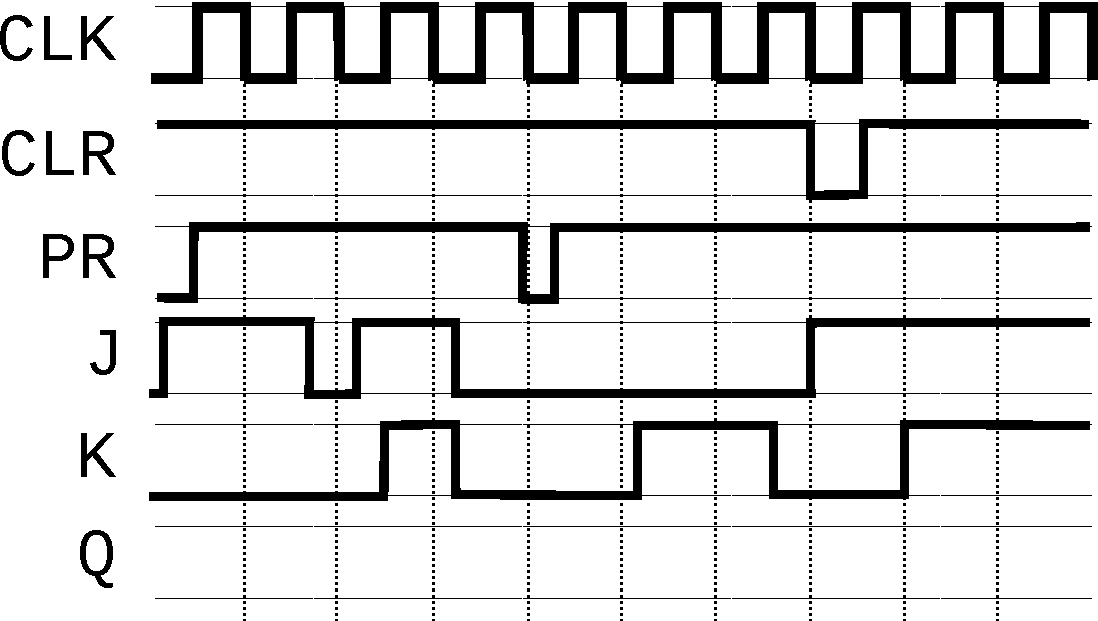
\includegraphics[scale=0.6]{sig2} \vspace*{4cm}
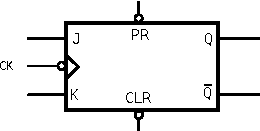
\includegraphics{fp-jk} \\
%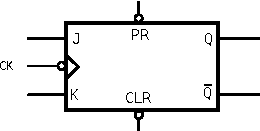
\includegraphics{fp-jk} \\ \vspace{15pt}
%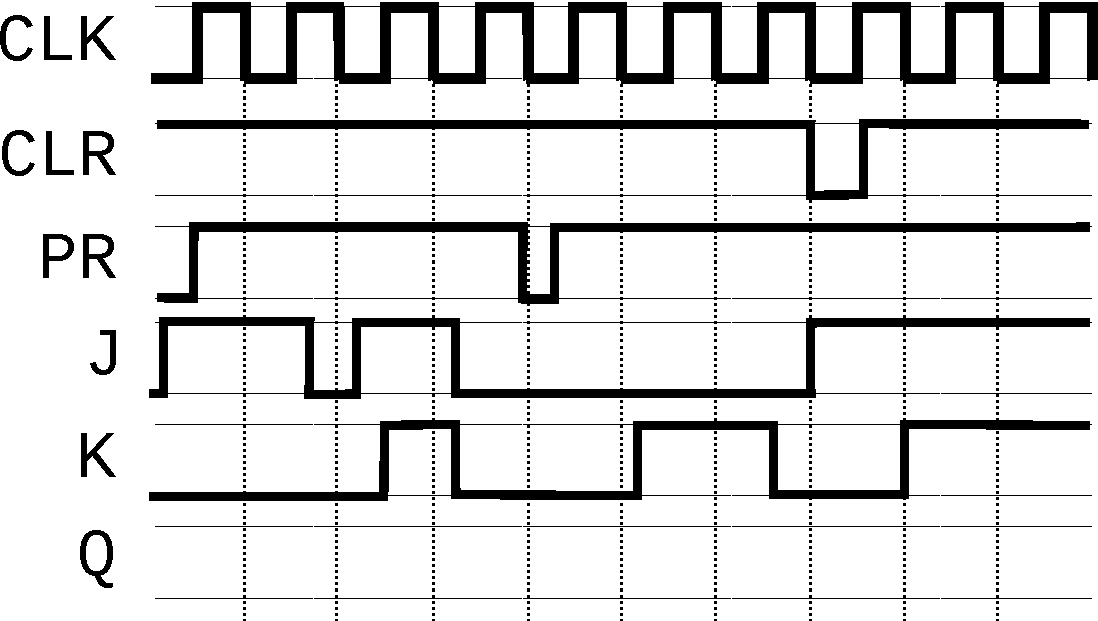
\includegraphics[scale=0.5]{sig2}
\end{center}
\end{multicols}

\end{document}

